\section{Vision Appendix}
\label{apx:vision}

\begin{figure}[h!]
    \caption{Technique for Finding Centroid}
    \label{bins}
    \centering
        \begin{enumerate}
            \item Go through frame pixel by pixel, if pixel is identified as yellow then place it one of five bins randomly.
            \item Calculate centroid of all five bins. See figure~\ref{vis2}.
            \item If the centroid of a bin does not lie on a yellow pixel then discard it, thus removing the noisy pixels.
            \item Take the mean of the remaining centroids and set this to be the centroid of the object, in this case the yellow T.  As seen in figure~\ref{vis3}.
            \item If all bins were discarded then keep the centroid where it was.
        \end{enumerate}
\end{figure}

\begin{figure}[h!]
  \caption{Centroiding being affected by noise}
  \label{vis1}
  \centering
    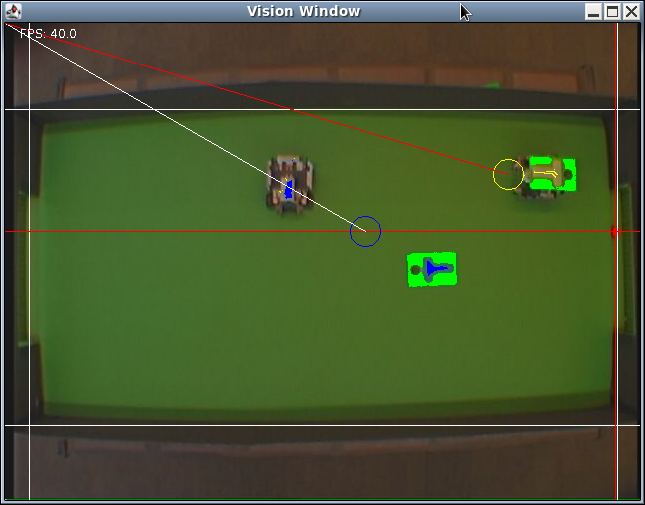
\includegraphics[width=0.5\textwidth]{randy_bins_before.png}
\end{figure}

\begin{figure}[h!]
  \caption{One centroid for each bin, indicated by pink dots}
  \label{vis2}
  \centering
    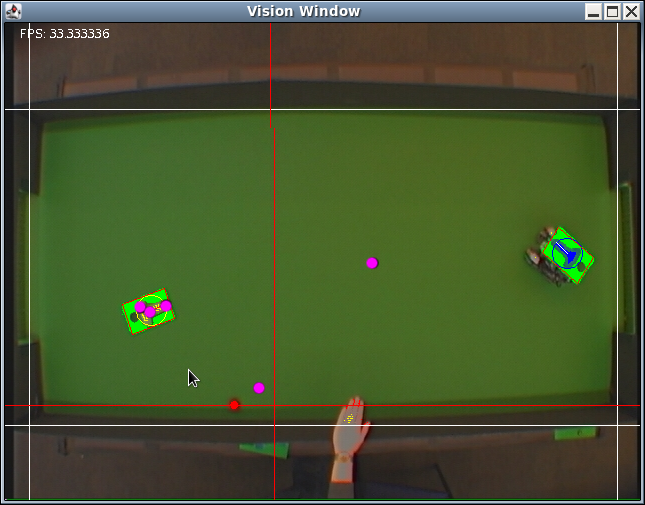
\includegraphics[width=0.5\textwidth]{randy_bins_after_mult.png}
\end{figure}

\begin{figure}[h!]
  \caption{Centroiding being unaffected by noise}
  \label{vis3}
  \centering
    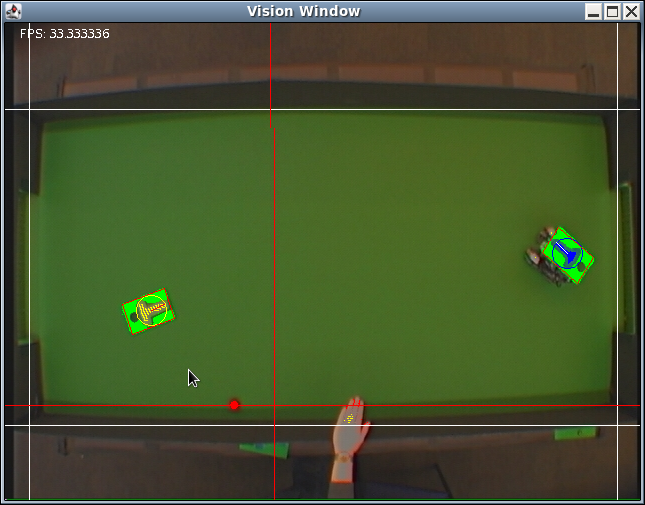
\includegraphics[width=0.5\textwidth]{randy_bins_after.png}
\end{figure}



%The label is so it can be dynamically refrenced from else where in the
%document
